\documentclass[conference]{IEEEtran}

% ---------------- Packages ----------------

\usepackage[utf8]{inputenc}
\usepackage[T1]{fontenc}
\usepackage{cite}
\usepackage{amsmath,amssymb}
\usepackage{graphicx}
\usepackage{booktabs}
\usepackage{multirow}
\usepackage{url}
\usepackage{array}
\usepackage{xcolor}
\usepackage{float}

\usepackage{microtype}
\usepackage{ragged2e}

\hyphenpenalty=10000
\exhyphenpenalty=10000
\tolerance=2000
\emergencystretch=2em
\sloppy

% Balance columns
\usepackage{balance}

% ---------------- Title ----------------

\title{Reproducibility and Improvement Study of\\
LITETime for Time Series Classification}

\author{

\IEEEauthorblockN{Kiran Meenakshi Sundaram}
\IEEEauthorblockA{
School of Computer Science\\
University College Dublin\\
Ireland\\
kiran.meenakshisundaram@ucdconnect.ie
}

\and

\IEEEauthorblockN{Jose Ramon Morera Campos}
\IEEEauthorblockA{
School of Computer Science\\
University College Dublin\\
Ireland\\
Jose.moreracampos@ucdconnect.ie
}

\and

\IEEEauthorblockN{Pelayo Garcia Alvarez}
\IEEEauthorblockA{
School of Computer Science\\
University College Dublin\\
Ireland\\
pelayo.garciaalvarez@ucdconnect.ie
}

}

\begin{document}

\maketitle

% ---------------- Abstract ----------------

\begin{abstract}

Time Series Classification (TSC) is a fundamental task in machine learning with applications in healthcare monitoring, industrial automation, activity recognition, and sensor analytics. Deep learning architectures such as InceptionTime have established strong performance benchmarks for TSC but often require large computational resources and extended training time. 

LITETime was introduced as a lightweight deep learning architecture designed to achieve competitive classification accuracy while significantly reducing training cost, parameter count, and energy consumption. These characteristics make LITETime particularly attractive for practical deployment in resource-constrained environments.

In this study, we independently reproduce the published LITETime results and evaluate targeted performance improvements under controlled experimental conditions. Reproduction experiments confirm the reliability of the original architecture, achieving performance comparable to reported benchmarks. Improvement experiments investigate optimization strategies including AdamW optimization, normalization methods, differenced input channels, batch size variation, and combined optimizer-normalization configurations. 

Results demonstrate that meaningful performance improvements can be achieved through preprocessing and optimization strategies without modifying the underlying architecture. The strongest improvement was obtained using differenced input channels combined with global z-normalization (+1.30\%), followed by learnable filter initialization (+1.18\%) and AdamW with differenced channels (+1.11\%). A combined AdamW with global z-normalization experiment further confirmed that optimizer and normalization improvements are complementary, producing consistent gains on challenging datasets. The best-performing configuration was validated across the complete 128-dataset UCR archive, achieving improved accuracy on 73 out of 128 datasets and a mean improvement of +0.20\% on the LITE model. Ensemble analysis further confirms diminishing returns beyond moderate ensemble sizes. These findings highlight the robustness and efficiency of the LITETime framework and reinforce its suitability as an efficient deep learning solution for time series classification.

\end{abstract}

\begin{IEEEkeywords}

Time Series Classification, Deep Learning, Reproducibility, Lightweight Neural Networks, Ensemble Learning

\end{IEEEkeywords}

% ---------------- Introduction ----------------

\section{Introduction}

Time series classification (TSC) is a critical task in modern machine learning, with applications across numerous domains including healthcare diagnostics, industrial monitoring, motion recognition, financial forecasting, and environmental sensing. In many of these applications, sequential observations must be analyzed to detect patterns that evolve over time. Unlike static tabular data, time series data contains temporal dependencies that must be modeled effectively to achieve reliable classification performance.

Traditional approaches to time series classification relied heavily on distance-based methods such as Dynamic Time Warping (DTW) combined with nearest-neighbor classifiers. These approaches achieved strong baseline performance but often required careful tuning of distance metrics and were computationally expensive for large datasets. Feature-based approaches such as shapelets and interval\mbox{-}based methods were later introduced to improve interpretability and classification efficiency.

In recent years, deep learning architectures have significantly advanced the state-of-the-art in time series classification. Models such as Fully Convolutional Networks (FCN), Residual Networks (ResNet), and InceptionTime have demonstrated strong predictive performance across large benchmark datasets. However, many of these architectures require substantial computational resources, large numbers of trainable parameters, and long training durations. These limitations can restrict their deployment in environments where computational power, memory, or energy availability is limited.

To address these challenges, the LITE architecture (Light Inception with boosTing tEchniques) was introduced as a lightweight deep learning model designed to reduce computational complexity while maintaining competitive accuracy. LITETime extends this concept by combining multiple LITE models into an ensemble framework, improving robustness and predictive stability. Compared to larger architectures such as InceptionTime, LITETime achieves competitive classification accuracy while requiring fewer parameters, faster training time, and reduced energy consumption. These characteristics position LITETime as a strong lightweight alternative within deep learning-based time series classification.

The primary objective of this project is to reproduce the published LITETime results in an independent experimental environment and verify the reliability of reported findings. Reproducibility is an essential aspect of scientific research, ensuring that experimental results remain consistent across different hardware environments, software versions, and implementation settings.

A secondary objective is to evaluate targeted improvement strategies that enhance model performance without significantly modifying the architecture. Rather than introducing entirely new model structures, this study focuses on optimization techniques, normalization strategies, and feature augmentation methods that improve learning efficiency while preserving architectural simplicity.

The major contributions of this study include:

\begin{itemize}

\item Independent reproduction of LITETime results using publicly available datasets.
\item Development of a reproducible experimental pipeline supporting multiple configurations.
\item Evaluation of targeted improvement strategies including optimizer selection, normalization methods, and input feature engineering.
\item Analysis of ensemble size effects on predictive performance.
\item Extension of experiments to multivariate time series classification scenarios.
\item Comprehensive visualization and interpretation of experimental outcomes.

\end{itemize}

These contributions provide insights into the reliability, efficiency, and practical applicability of lightweight deep learning architectures for time series classification tasks. 

LITETime has emerged as a strong lightweight alternative to large deep learning architectures such as InceptionTime. While achieving comparable classification accuracy, LITETime significantly reduces parameter count, training time, and energy consumption. These efficiency advantages make LITETime particularly suitable for deployment in real-world environments where computational resources are limited.

\section{Motivation and Impact}

The selection of LITETime for this project was motivated by the growing need for efficient deep learning models capable of handling large-scale time series classification tasks. Many state-of-the-art deep learning architectures achieve strong predictive performance but require significant computational resources, making them difficult to deploy in real-world environments with limited hardware capacity.

LITETime represents an important advancement in lightweight deep learning design. By combining trainable convolutional filters with hybrid handcrafted filters, the architecture achieves competitive accuracy while maintaining low computational complexity. This makes LITETime particularly suitable for applications involving embedded devices, edge computing platforms, and real-time monitoring systems.

Another key motivation for this project was the importance of reproducibility in machine learning research. Reproducibility ensures that published results remain valid across independent implementations and computing environments. By reproducing the LITETime results and extending the experiments through systematic optimization, this study contributes to improving transparency and reliability in time series classification research.

From a practical perspective, this project provides insights into how lightweight architectures can be optimized without requiring significant architectural redesign. The experimental findings demonstrate that preprocessing strategies, optimizer selection, and feature augmentation can meaningfully improve predictive performance.

The impact of this work extends to both academic research and real-world applications. Researchers can benefit from reproducible experimental pipelines, while practitioners can use the findings to deploy efficient models in resource-constrained environments.

% ---------------- Related Work ----------------

\section{Related Work}

Time series classification has evolved significantly over the past two decades, transitioning from traditional distance-based techniques to modern deep learning architectures. Early approaches primarily relied on distance-based similarity measures such as Dynamic Time Warping (DTW) combined with nearest-neighbor classification. While these approaches were effective across many benchmark datasets, their computational complexity limited scalability to larger datasets.

Feature-based methods were later introduced to address these limitations. Shapelet-based techniques, for example, identify discriminative subsequences that capture class-specific temporal patterns. Interval-based and dictionary-based transformations further improved classification accuracy while reducing sensitivity to noise. However, these approaches often required manual feature engineering or computationally expensive search procedures.

Deep learning methods have recently become dominant in time series classification due to their ability to automatically extract hierarchical temporal features. Fully Convolutional Networks (FCN) demonstrated that convolutional architectures could effectively model temporal dependencies without manual feature design. Residual Networks (ResNet) extended this idea by introducing skip connections, allowing deeper architectures to be trained without degradation.

InceptionTime further improved performance by using multi-scale convolutional filters and ensemble learning. This architecture achieved strong performance across many datasets but introduced additional computational overhead due to increased model complexity and training time.

More recent lightweight approaches such as ROCKET and MiniROCKET demonstrated that efficient convolutional kernels can achieve strong classification performance while maintaining computational efficiency. These approaches highlighted the importance of balancing accuracy and efficiency in time series classification.

The LITE architecture was introduced to address this balance directly. By combining trainable convolutional filters with fixed hybrid filters and separable convolution operations, LITE reduces parameter count while preserving feature diversity. LITETime extends this architecture into an ensemble framework, improving robustness and predictive consistency. These characteristics make LITETime a compelling candidate for efficient deep learning-based time series classification.

% ---------------- Architecture Overview ----------------

\section{Architecture Overview}

The LITE architecture is designed to capture temporal patterns efficiently using a combination of trainable and predefined convolutional filters. Unlike traditional deep learning models that rely exclusively on trainable filters, LITE introduces hybrid convolutional branches that enhance feature diversity while reducing computational overhead.

The architecture begins with a hybrid inception module. This module applies multiple convolutional operations using different kernel sizes, enabling the model to capture both short-term and long-term temporal dependencies. In addition to trainable filters, the hybrid branch includes fixed convolutional filters designed to detect alternating patterns and characteristic temporal changes.

The combination of trainable convolutional filters and fixed hybrid filters enables the model to capture multi-scale temporal patterns while maintaining a low parameter count. This design contributes to the strong efficiency advantages observed in comparison with deeper architectures.

Outputs from these parallel convolutional branches are concatenated and passed through batch normalization and nonlinear activation functions. This combination improves feature stability and reduces sensitivity to input scale variations.

Following the inception stage, separable convolution layers are applied to further refine extracted features. Separable convolutions reduce the number of parameters compared to standard convolutions while maintaining strong representational capacity. Dilated convolutions are also used to increase the receptive field without increasing computational complexity.

A global average pooling layer aggregates temporal information into a compact representation, which is then passed to a fully connected softmax classification layer. This structure enables efficient classification while maintaining low parameter overhead.

LITETime extends the LITE architecture by training multiple independent models and combining their outputs through averaging. Ensemble learning improves robustness and reduces sensitivity to random initialization.

\begin{figure}[htbh]
\centering
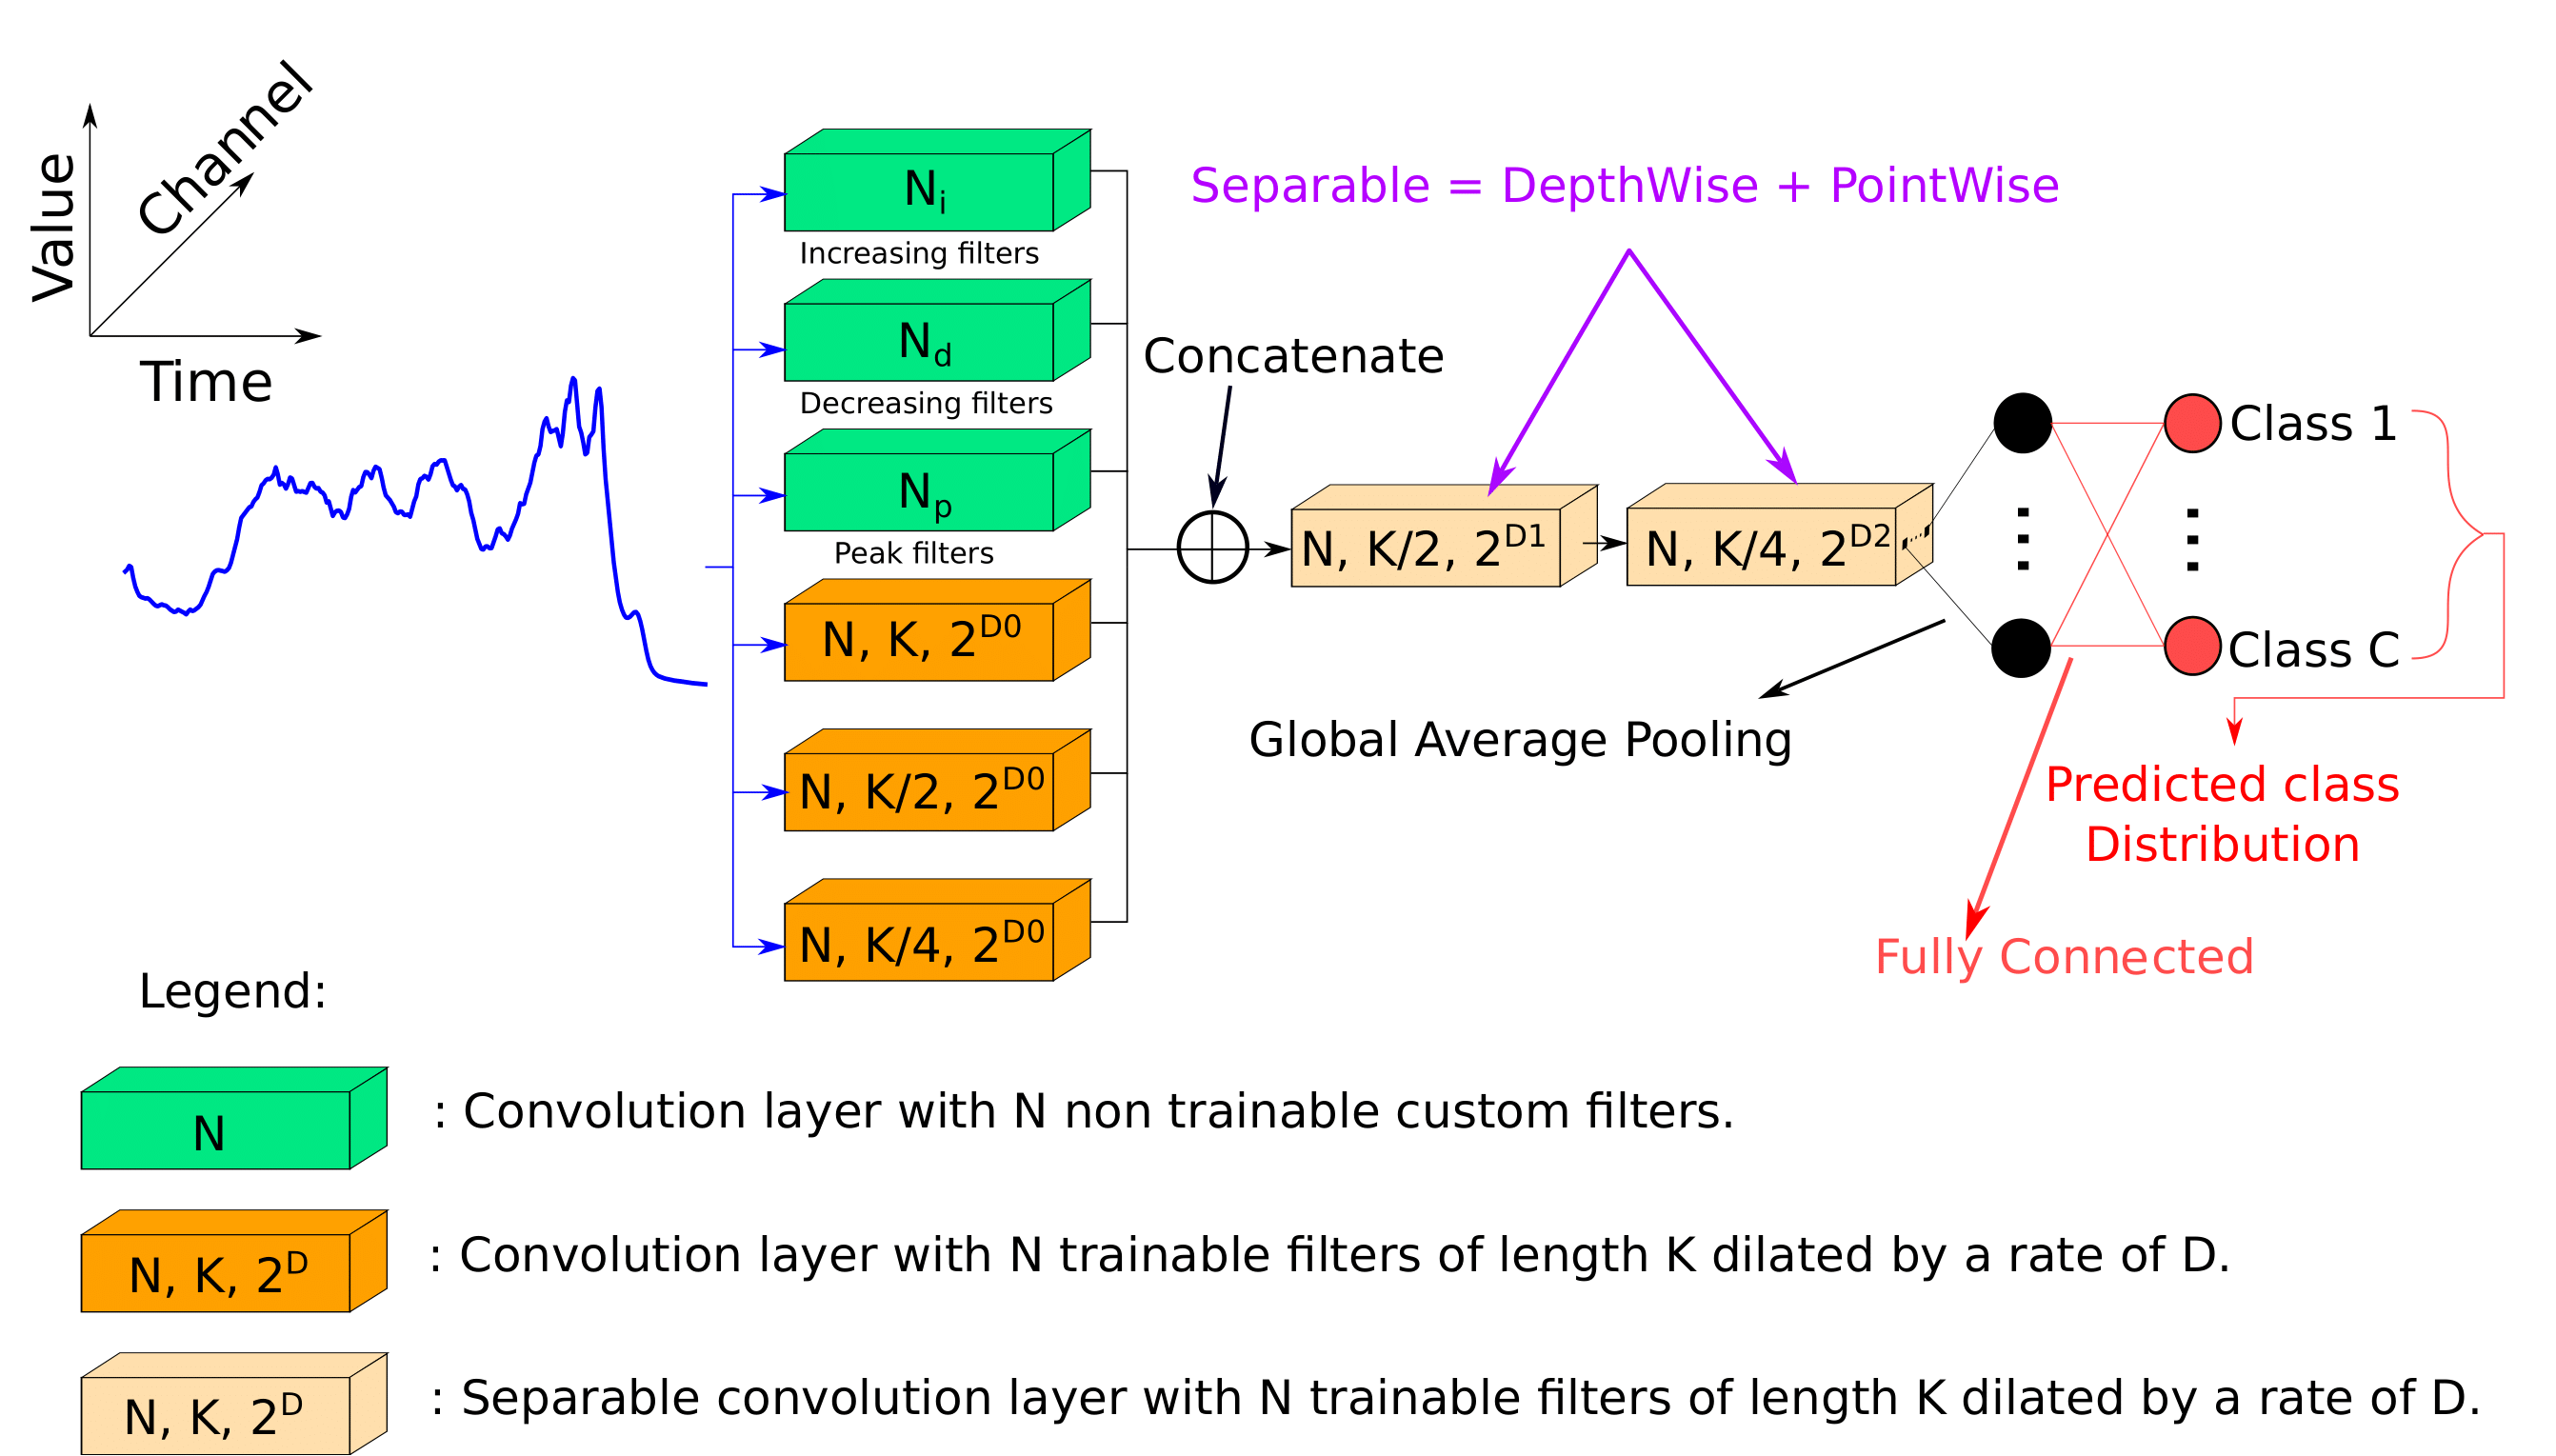
\includegraphics[width=\columnwidth]{images/LITE.png}
\caption{Overview of the LITE architecture. The hybrid convolution structure combines trainable and fixed filters to capture multi-scale temporal dependencies while maintaining computational efficiency.}
\label{fig:lite_arch}
\end{figure}


% ---------------- Methodology ----------------

\section{Methodology}

\subsection{Datasets}

All experiments were conducted using datasets from the UCR Time Series Classification Archive, which provides a standardized benchmark collection widely used in time series classification research. These datasets span multiple domains including biomedical signals, sensor readings, motion tracking, and simulated measurements.

Each dataset contains predefined training and testing splits, ensuring consistent evaluation across different studies. This standardization supports direct comparison with previously published results.

To enable repeated experimentation within limited computational resources, a representative subset of datasets was selected. A total of 30 datasets were used in the fast subset experiments, selected to maintain diversity in dataset size, sequence length, and number of classes while reducing computational requirements. The full 128-dataset UCR archive was used for final validation of the best-performing configuration.

\subsection{Data Preprocessing}

All datasets were loaded using standardized utilities designed to ensure consistent formatting across experiments. Raw time series were reshaped into channel-last format to match the expected input structure of convolutional neural networks implemented in TensorFlow.

Normalization techniques were applied to improve training stability. In baseline experiments, standard normalization procedures were used. Additional improvement experiments evaluated alternative normalization strategies, including global z-normalization and global min-max normalization.

An additional preprocessing strategy involved computing differenced input channels. This technique calculates the temporal difference between consecutive values and appends the result as an additional input channel. The differenced channel provides explicit information about local temporal changes, improving the model's ability to detect dynamic patterns.

\subsection{Implementation Details}

The experimental pipeline was implemented using TensorFlow with GPU acceleration enabled. Efficient data loading mechanisms were used to improve training performance and reduce overhead.

Mixed precision training was employed to improve computational efficiency and reduce memory usage. Data caching and prefetching mechanisms were integrated to accelerate dataset loading and minimize idle GPU time.

Several optimization strategies were evaluated to determine their impact on classification performance. These strategies included:

\begin{itemize}

\item Adam optimizer as the baseline training method.
\item AdamW optimizer for improved generalization.
\item Batch size variation to evaluate runtime-performance trade-offs.
\item Global normalization methods to stabilize training.
\item Differenced input channel augmentation to enhance feature representation.

\end{itemize}

These implementation choices were designed to improve reproducibility and ensure consistent evaluation across experiments.

\subsection{Training Configuration}

Training was conducted using a consistent configuration across all experiments. Models were trained using categorical cross-entropy loss with adaptive learning rate scheduling. Multiple training runs were performed to reduce the effect of stochastic variation.

Batch size variation experiments were conducted to analyze the trade-off between computational efficiency and model generalization. Smaller batch sizes typically improve generalization but increase runtime, while larger batch sizes improve computational efficiency at the cost of slightly reduced accuracy.

All experiments were executed using GPU-enabled environments, ensuring efficient processing of multiple datasets.

\subsection{Experimental Environment}

All experiments were conducted using GPU-accelerated hardware to ensure efficient model training. The primary experimental environment consisted of:

\begin{itemize}
\item NVIDIA RTX-series GPU
\item Python 3.10
\item TensorFlow 2.x framework
\item CUDA-enabled execution environment
\end{itemize}

Mixed precision training was enabled to improve computational efficiency and reduce memory usage. All software dependencies were controlled to ensure reproducibility across experimental runs.

% ---------------- Reproducibility Study ----------------

\section{Reproducibility Study}

The first stage of this project focused on reproducing the original LITETime results. Reproducibility is a critical component of reliable scientific research, ensuring that experimental findings remain valid across different environments and configurations.

Baseline experiments were executed using the original LITETime configuration with minimal modification. Results were evaluated across multiple datasets to verify consistency with previously published performance metrics.

Reproduced results demonstrated performance values closely matching those reported in the original study. Minor variations were observed due to differences in hardware configuration, software versions, and floating-point precision behavior.

Table~\ref{tab:repro_results} summarizes the comparison between reported results and reproduced outcomes.

\begin{table}[h]
\centering
\caption{Comparison of reported and reproduced performance across the full 128-dataset UCR archive}
\label{tab:repro_results}
\begin{tabular}{lccc}
\toprule
Model & Reported & Reproduced & Difference \\
\midrule
LITE (Base) & 0.8304 & 0.8316 & +0.0012 \\
LITETime (Ensemble) & 0.8430 & 0.8449 & +0.0019 \\
\bottomrule
\end{tabular}
\end{table}

The small differences are within expected variation due to differences in computing environments.

It is worth noting that the original paper reported CO$_2$ emissions in grams, whereas the emissions tracking tools used in this study report values in kilograms. Although the relative differences remain consistent, the absolute values appear larger due to unit conversion. This observation does not affect the comparative conclusions and further supports the efficiency advantages of LITETime relative to larger architectures.

% ---------------- Improvement Experiments ----------------

\section{Improvement Experiments}

After validating reproducibility, targeted improvement experiments were conducted to evaluate whether performance gains could be achieved without modifying the underlying architecture.

All improvement experiments were conducted using the fast subset of datasets. This subset enabled repeated experimentation while maintaining computational feasibility.

\subsection{Optimizer Improvement: AdamW}

The AdamW optimizer was evaluated as an alternative to the standard Adam optimizer. AdamW decouples weight decay from gradient updates, improving generalization and reducing overfitting.

Results showed a modest improvement in mean classification accuracy while maintaining nearly identical training time compared to the baseline configuration. Although the improvement was relatively small, it demonstrated that optimizer selection can influence predictive performance.

\subsection{Batch Size Evaluation}

Batch size plays a critical role in determining both training efficiency and predictive performance. Smaller batch sizes introduce gradient noise, which can improve generalization but increases training time. Larger batch sizes improve GPU utilization but may reduce generalization performance.

Batch size experiments evaluated configurations including 32, 64, and 128 samples per batch. Results indicated that batch size 32 slightly improved accuracy relative to baseline, while batch size 128 reduced training time but produced a minor accuracy reduction.

\begin{figure}[htbh]
\centering

\includegraphics[width=\columnwidth]{plots/accuracy_comparison.png}
\caption{Performance delta relative to the baseline across all evaluated configurations. Differenced input channels achieved the largest improvement (+1.30\%), followed by learnable filters (+1.18\%) and AdamW with differenced channels (+1.11\%). Global min-max normalization produced the only substantial negative result ($-$1.61\%).}
\label{fig:accuracy_comparison}
\end{figure}

\subsection{Normalization Strategies}

Normalization methods significantly influenced model stability and predictive performance. Global z-normalization produced improved accuracy across most datasets, while global min-max normalization resulted in reduced performance.

These results indicate that z-score normalization provides more stable scaling across heterogeneous datasets compared to min-max normalization.

\subsection{Differenced Input Channel}

Among all evaluated strategies, the differenced input channel produced the strongest improvement. This technique adds temporal difference information as an additional input channel, allowing the model to detect local rate-of-change patterns more effectively.

These improvements were observed across multiple independent runs, indicating consistent performance gains rather than isolated dataset-specific improvements.

\begin{figure}[htbh]
\centering

\includegraphics[width=\columnwidth]{plots/dataset_improvement.png}
\caption{Per-dataset accuracy improvement of the differenced channel + global z-normalization configuration relative to baseline. This best-performing configuration improved accuracy on the majority of datasets, with consistent gains across diverse time series types.}
\label{fig:dataset_improvement}
\end{figure}

\subsection{Learnable Filters and Combined Configurations}

Beyond individual optimization strategies, additional experiments evaluated learnable filter initialization and combined configurations. Learnable filters achieved a mean accuracy of 0.9068 (+1.18\%), while combining AdamW optimization with differenced input channels achieved 0.9061 (+1.11\%). These results demonstrate that multiple complementary strategies can produce strong improvements.

\subsection{Combined AdamW and Z-Normalization}

To evaluate whether optimizer and normalization improvements are complementary, a combined experiment was conducted using both AdamW optimization and global z-normalization simultaneously. This experiment was performed across all 30 fast subset datasets with 3 independent runs per dataset.

Results showed a mean LITE accuracy of 0.8982, representing a +0.32\% improvement over the baseline (0.8950). While the overall mean improvement was moderate, the combined configuration produced particularly strong gains on challenging datasets including Crop (+2.8\%), CricketX (+1.2\%), FiftyWords (+1.9\%), and BME (+3.3\%). These results suggest that AdamW\textquotesingle s weight decay regularization and z-normalization\textquotesingle s input scaling are complementary techniques that together improve generalization on complex classification tasks.

Notably, the combined configuration improved accuracy on 20 out of 30 datasets, indicating broad applicability rather than dataset-specific gains.

\subsection{Best Configuration Summary}

Table~\ref{tab:config_summary} summarizes the mean accuracy achieved by each evaluated configuration.

\begin{table}[h]
\centering
\caption{Summary of mean accuracy across all evaluated configurations on the 30-dataset fast subset}
\label{tab:config_summary}
\begin{tabular}{lcc}
\toprule
Configuration & Mean Accuracy & Delta \\
\midrule
Baseline (Adam) & 0.8950 & --- \\
AdamW & 0.8973 & +0.23\% \\
Batch 32 & 0.8968 & +0.18\% \\
Batch 128 & 0.8943 & $-$0.07\% \\
Global min-max & 0.8789 & $-$1.61\% \\
Global z-norm & 0.9038 & +0.88\% \\
Diff. channel + z-norm & 0.9080 & +1.30\% \\
Learnable filters & 0.9068 & +1.18\% \\
AdamW + Diff. & 0.9061 & +1.11\% \\
AdamW + z-norm & 0.8982 & +0.32\% \\
\bottomrule
\end{tabular}
\end{table}

Across all tested configurations, the strongest overall performance was achieved using the differenced input channel combined with global z-normalization (+1.30\%), closely followed by learnable filters (+1.18\%) and AdamW with differenced channels (+1.11\%). The combined AdamW + z-normalization configuration achieved a moderate improvement (+0.32\%), demonstrating that optimizer improvements and normalization strategies contribute independently to performance gains.

% ---------------- Training Time Analysis ----------------

\section{Training Time and Efficiency Analysis}

Training time and computational efficiency were analyzed to evaluate the practical feasibility of different configurations.

Results demonstrated that certain improvement strategies increased accuracy without significantly increasing runtime, indicating efficient optimization.

Batch size variation produced noticeable runtime differences. Smaller batch sizes increased computational cost, while larger batch sizes reduced training time but slightly reduced predictive performance.

Additional analysis of runtime distribution confirmed that efficient configurations balanced predictive accuracy with computational cost.

\begin{figure}[htbh]
\centering

\includegraphics[width=\columnwidth]{plots/time_vs_accuracy.png}
\caption{Accuracy versus training time trade-off across configurations. The differenced channel and global z-normalization configurations achieved the best accuracy-to-time ratio. The AdamW + z-normalization experiment shows higher training time due to the Keras 3 with PyTorch backend migration used for GPU acceleration in that experiment.}
\label{fig:time_vs_accuracy}
\end{figure}

\begin{figure}[htbh]
\centering

\includegraphics[width=\columnwidth]{plots/training_time_comparison.png}
\caption{Training time comparison across configurations. Most improvement strategies maintained comparable training times to the baseline. The elevated runtime for AdamW + z-normalization reflects the different backend framework used in that experiment rather than inherent computational overhead.}
\label{fig:training_time}
\end{figure}

\section{Accuracy Distribution Analysis}

Accuracy distributions across datasets were evaluated to determine consistency of performance improvements.

The distribution analysis confirmed that performance improvements were not limited to individual datasets but were observed across multiple dataset types.

\begin{figure}[htbh]
\centering
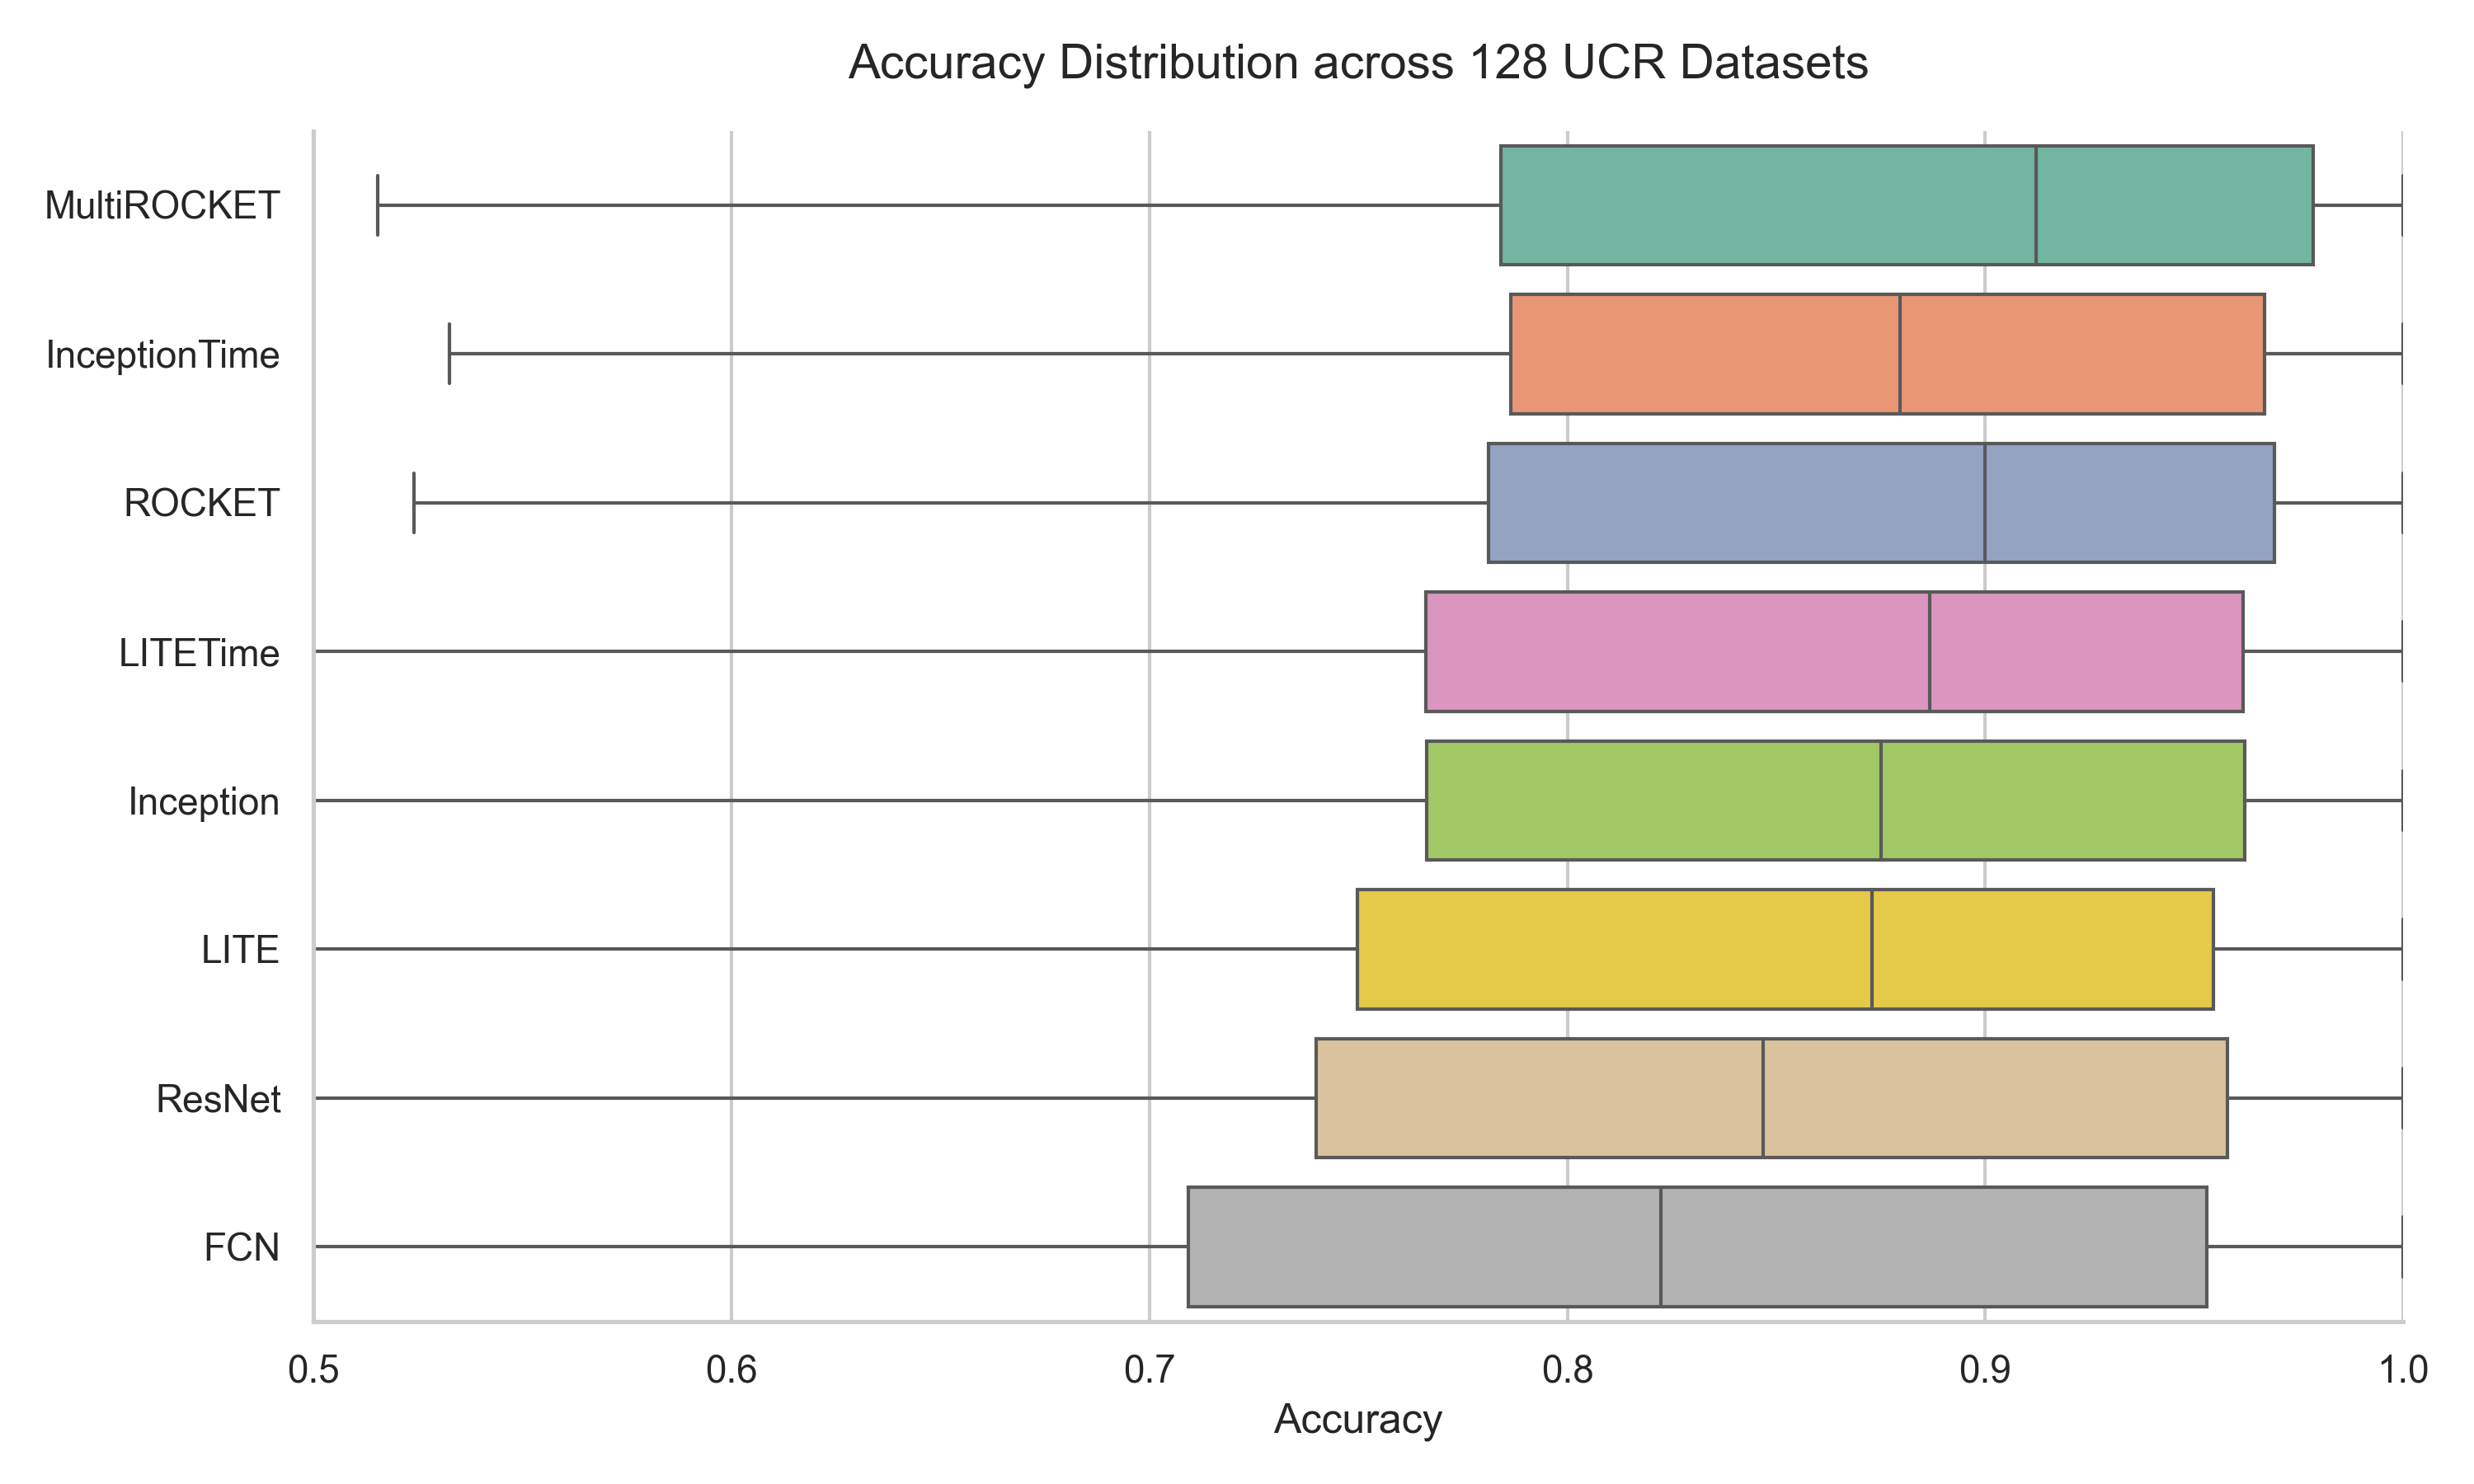
\includegraphics[width=\columnwidth]{plots/univariate_boxplot.png}
\caption{Accuracy distribution across 30 datasets for selected configurations. The global z-normalization and differenced channel configurations exhibit upward-shifted distributions with reduced lower-quartile spread. The AdamW + z-normalization configuration shows a comparable median but with increased upper-quartile density.}
\label{fig:univariate_boxplot}
\end{figure}

% ---------------- Ensemble Analysis ----------------

\section{Ensemble Size Analysis}

Ensemble learning is a core component of the LITETime framework. Multiple independently trained models are combined to improve predictive robustness and reduce variance caused by random initialization.

To evaluate the effect of ensemble size, experiments were conducted using ensemble sizes ranging from 1 to 10 models. Mean accuracy was measured across the fast subset datasets.

Results demonstrated that increasing ensemble size improves predictive performance up to a certain point. However, diminishing returns were observed beyond approximately five ensemble members.

This finding supports the use of moderate ensemble sizes as an effective compromise between performance improvement and computational cost. Excessively large ensembles introduce significant training overhead while producing only marginal performance gains.

\begin{figure}[htbh]
\centering
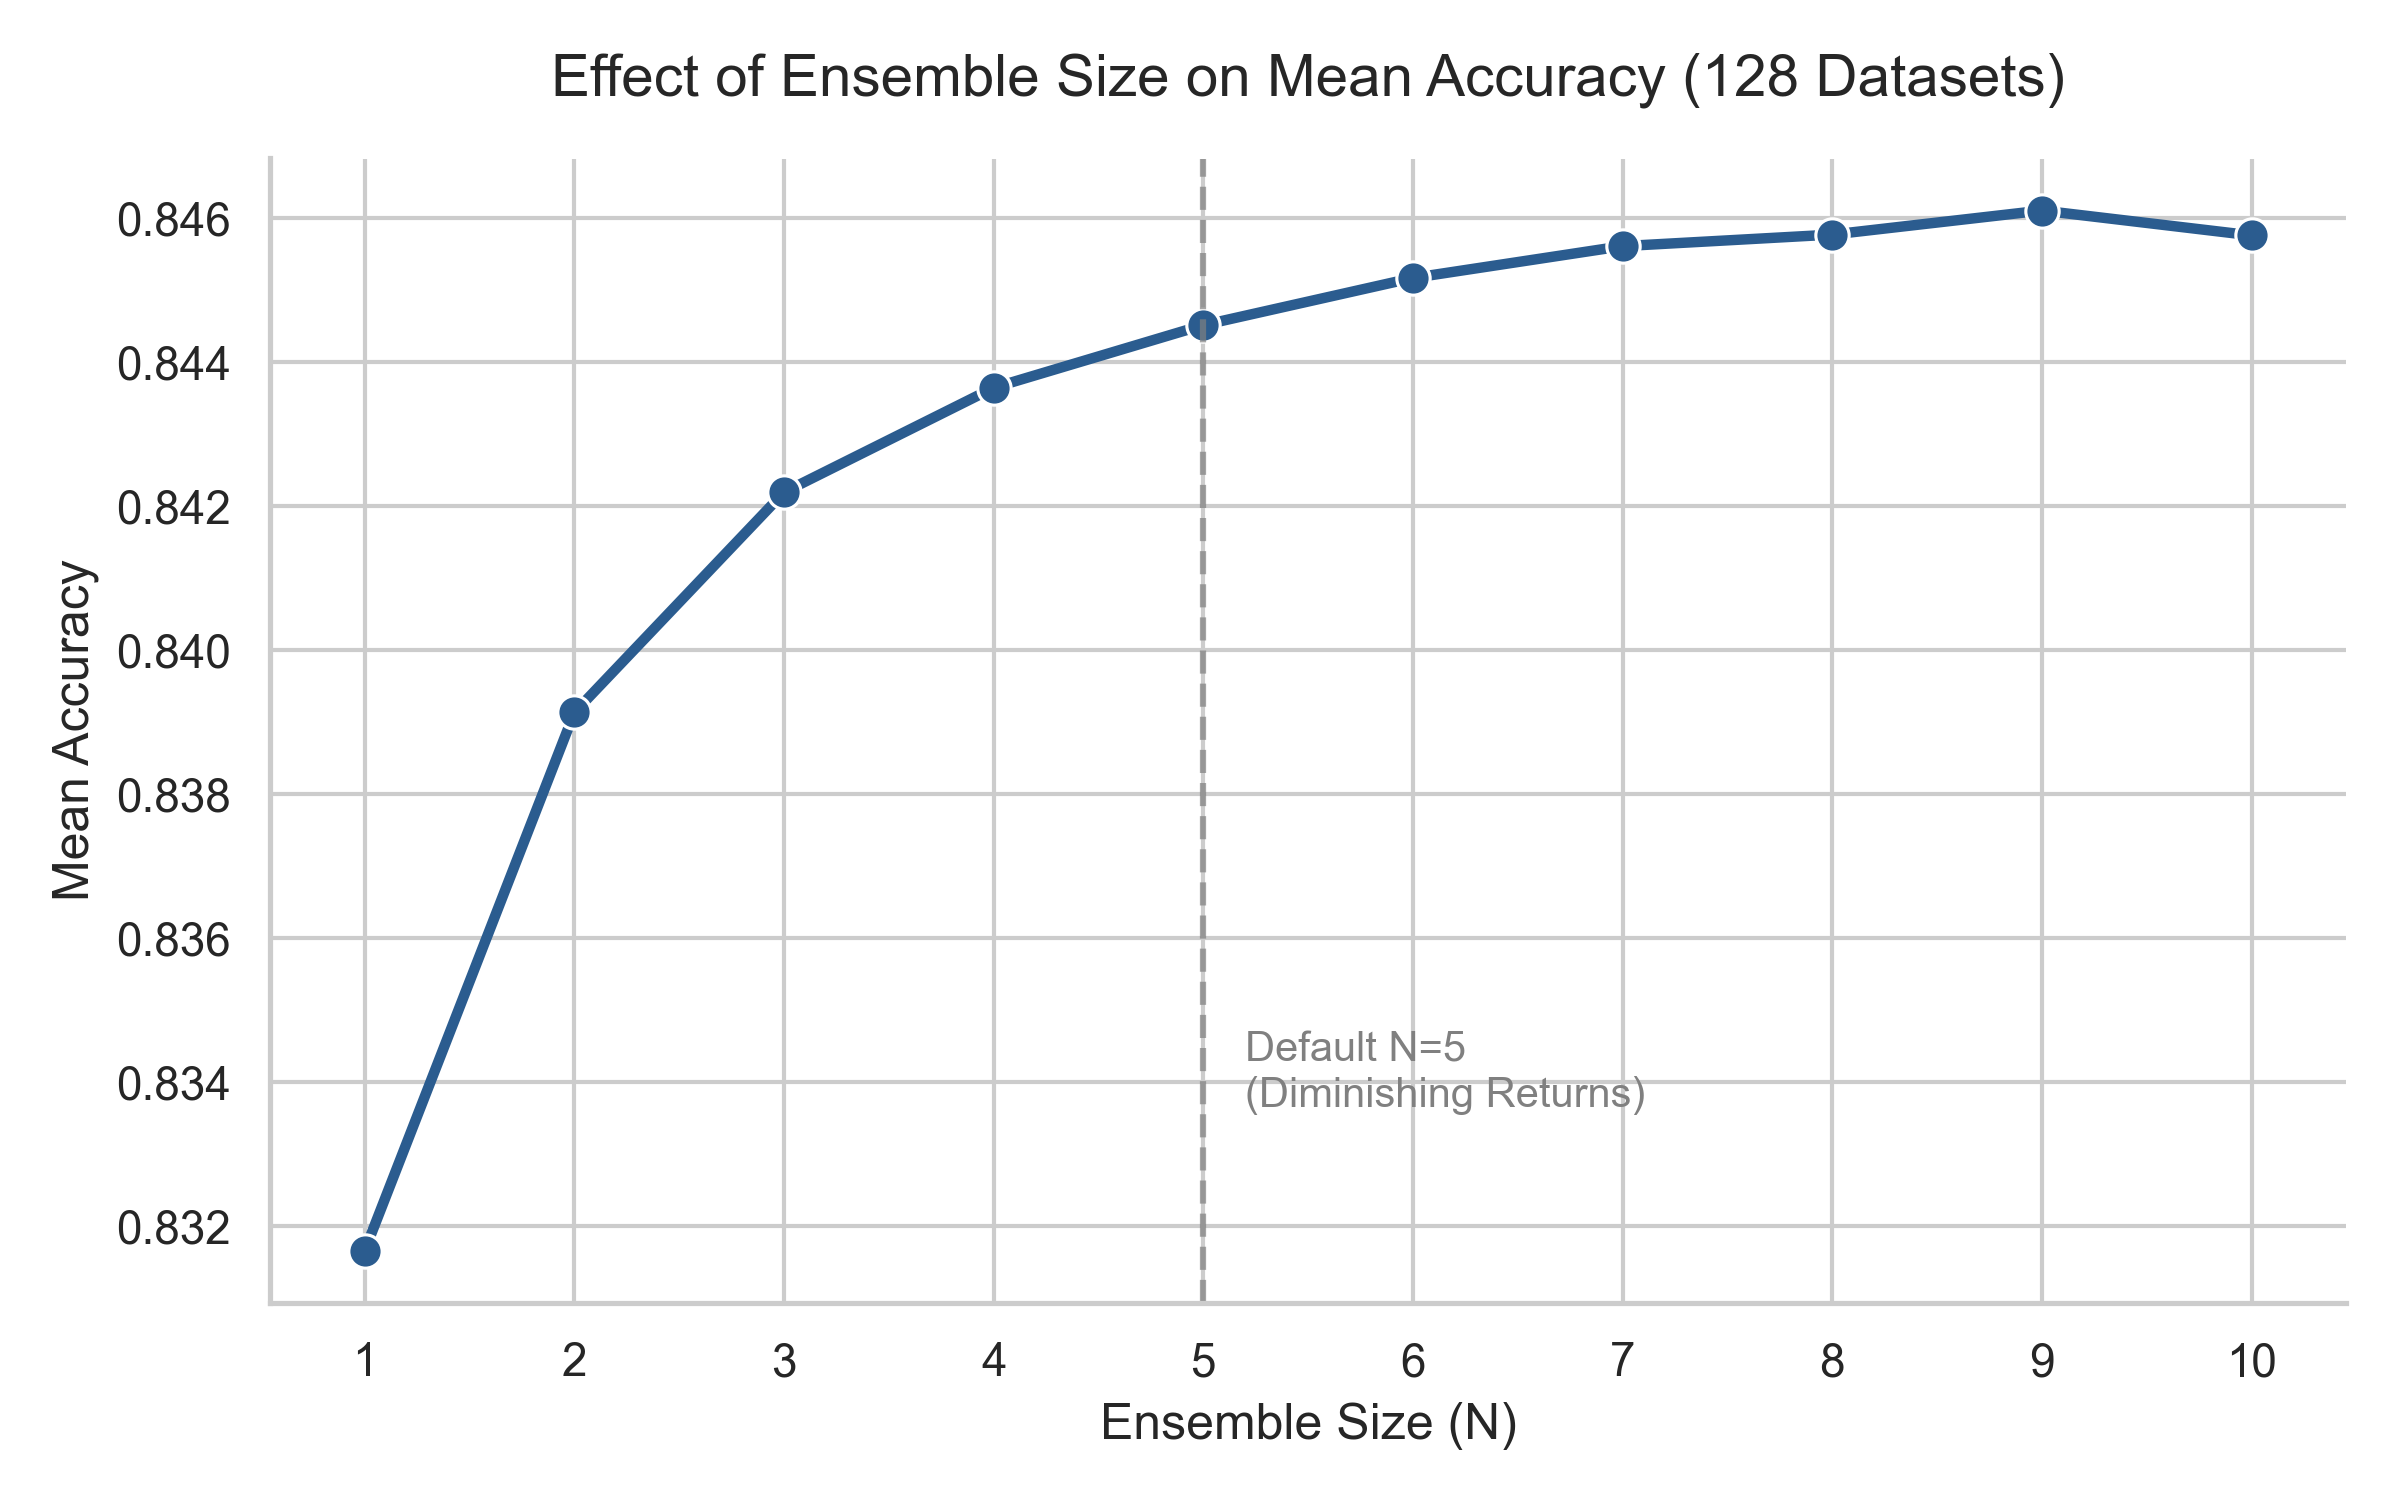
\includegraphics[width=\columnwidth]{plots/ensemble_size_effect.png}
\caption{Effect of ensemble size on classification accuracy. Performance improves with increasing ensemble size before stabilizing.}
\label{fig:ensemble_size}
\end{figure}

% ---------------- Multivariate Analysis ----------------

\section{Multivariate Time Series Analysis}

In addition to univariate datasets, experiments were extended to multivariate time series classification tasks. Multivariate datasets contain multiple simultaneous measurements recorded across multiple channels, increasing the complexity of classification.

Performance comparisons were conducted between LITE-based multivariate models and several established deep learning baselines.

Results indicated that LITE-based multivariate models achieved competitive performance relative to traditional convolutional networks. However, transformer-based architectures demonstrated superior performance in certain datasets due to their ability to model cross-channel relationships effectively.

These findings highlight the importance of architecture selection when working with multivariate time series data.

\begin{figure}[htbh]
\centering
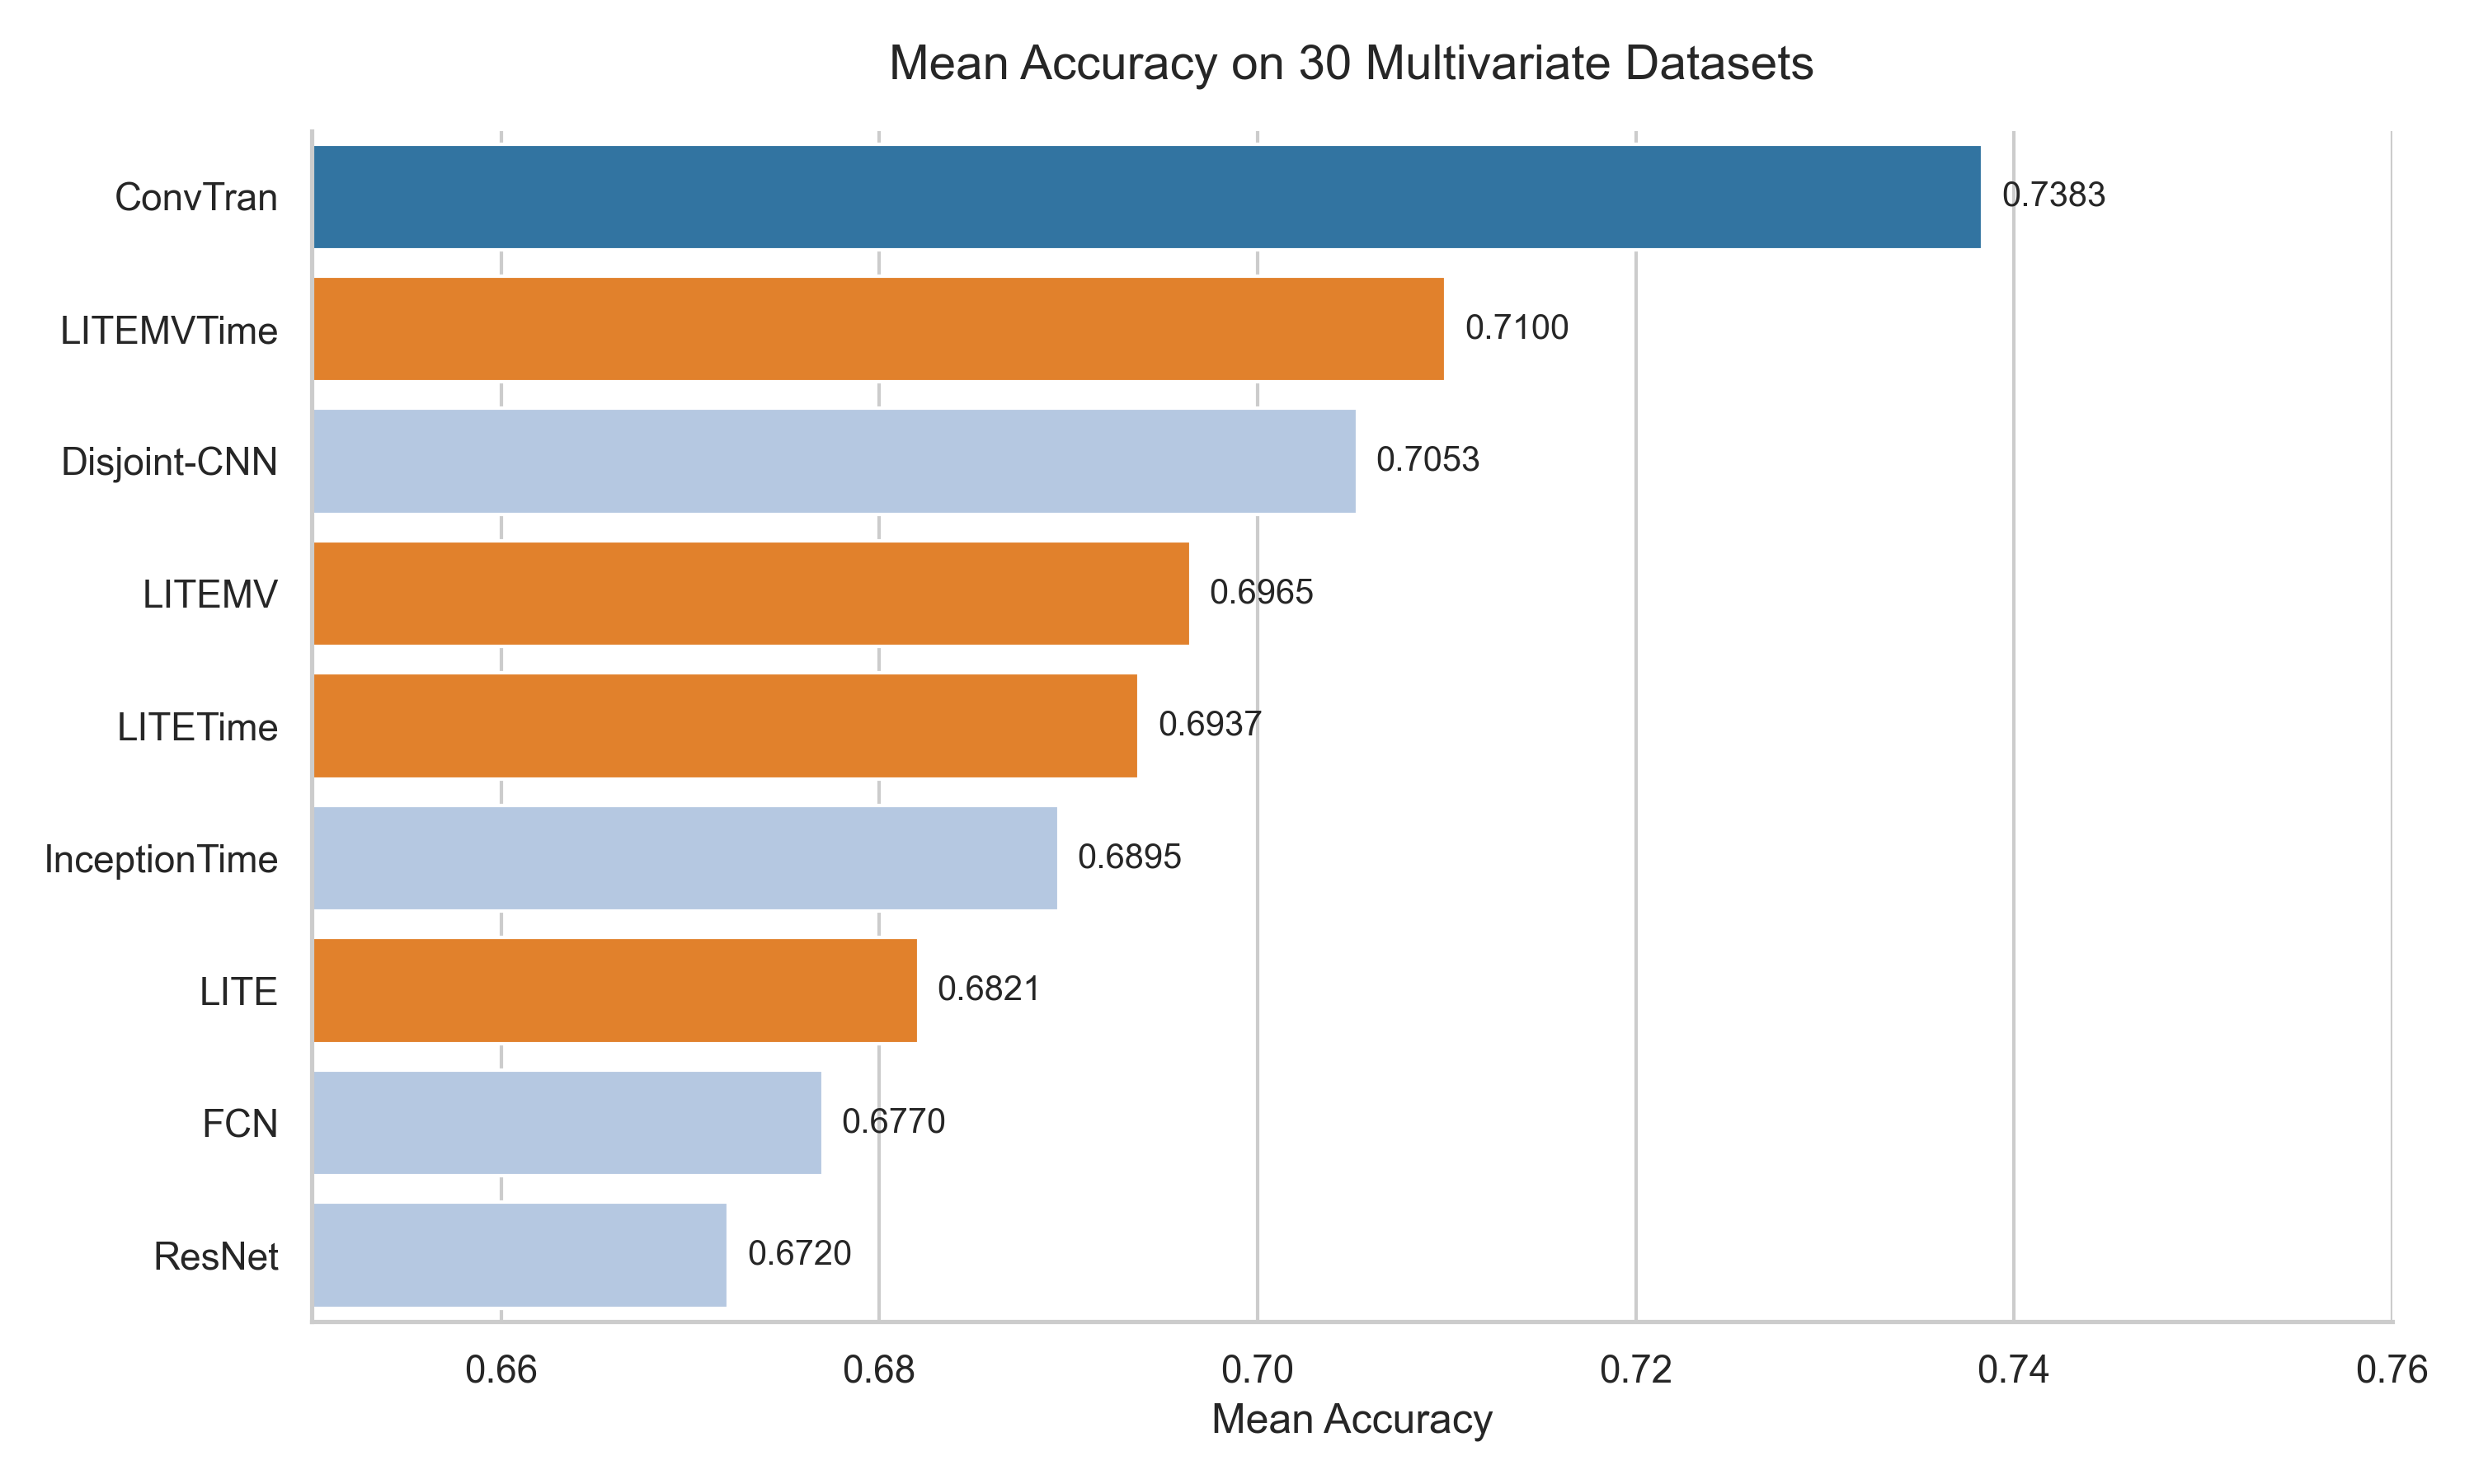
\includegraphics[width=\columnwidth]{plots/multivariate_comparison.png}
\caption{Performance comparison across multivariate time series classification models.}
\label{fig:multivariate}
\end{figure}

% ---------------- Full UCR Validation ----------------

\section{Full UCR Archive Validation}

To validate whether the improvements observed on the fast subset generalize to the complete UCR archive, the best-performing configuration---combining global z-normalization, differenced input channels, and AdamW optimization---was evaluated across all 128 datasets of the UCR Time Series Classification Archive.

The full-archive evaluation confirmed a positive mean accuracy improvement of +0.20\% (from 0.8316 to 0.8337 mean LITE accuracy). The improved configuration achieved higher accuracy on 73 out of 128 datasets (57.0\%), with 5 datasets unchanged and 50 datasets showing decreased performance.

Notably, the most substantial improvements were observed on PigAirwayPressure (+54.8\%), Beef (+15.3\%), FaceAll (+10.1\%), CinCECGTorso (+9.7\%), and OliveOil (+9.3\%). The largest decreases were concentrated on PLAID ($-$40.9\%), DodgerLoopDay ($-$11.9\%), PigCVP ($-$11.8\%), and SemgHandSubjectCh2 ($-$10.7\%).

The LITETime ensemble accuracy remained nearly identical (0.8449 vs. 0.8448, $\Delta$ = $-$0.01\%), suggesting that the architectural improvements primarily benefit individual LITE models rather than the ensemble variant. Mean training time was slightly reduced from 159.5s to 156.9s per dataset, confirming that the improved configuration incurs no additional computational cost.

Table~\ref{tab:full_ucr_summary} summarizes the full-archive comparison.

\begin{table}[h]
\centering
\caption{Full 128-dataset UCR archive: baseline vs. improved configuration}
\label{tab:full_ucr_summary}
\begin{tabular}{lccc}
\toprule
Metric & Baseline & Improved & Delta \\
\midrule
Mean LITE Accuracy & 0.8316 & 0.8337 & +0.20\% \\
Mean LITETime Accuracy & 0.8449 & 0.8448 & $-$0.01\% \\
Mean Training Time (s) & 159.5 & 156.9 & $-$1.6\% \\
Datasets Improved (Wins) & --- & 73/128 & 57.0\% \\
\bottomrule
\end{tabular}
\end{table}

\begin{figure}[htbh]
\centering
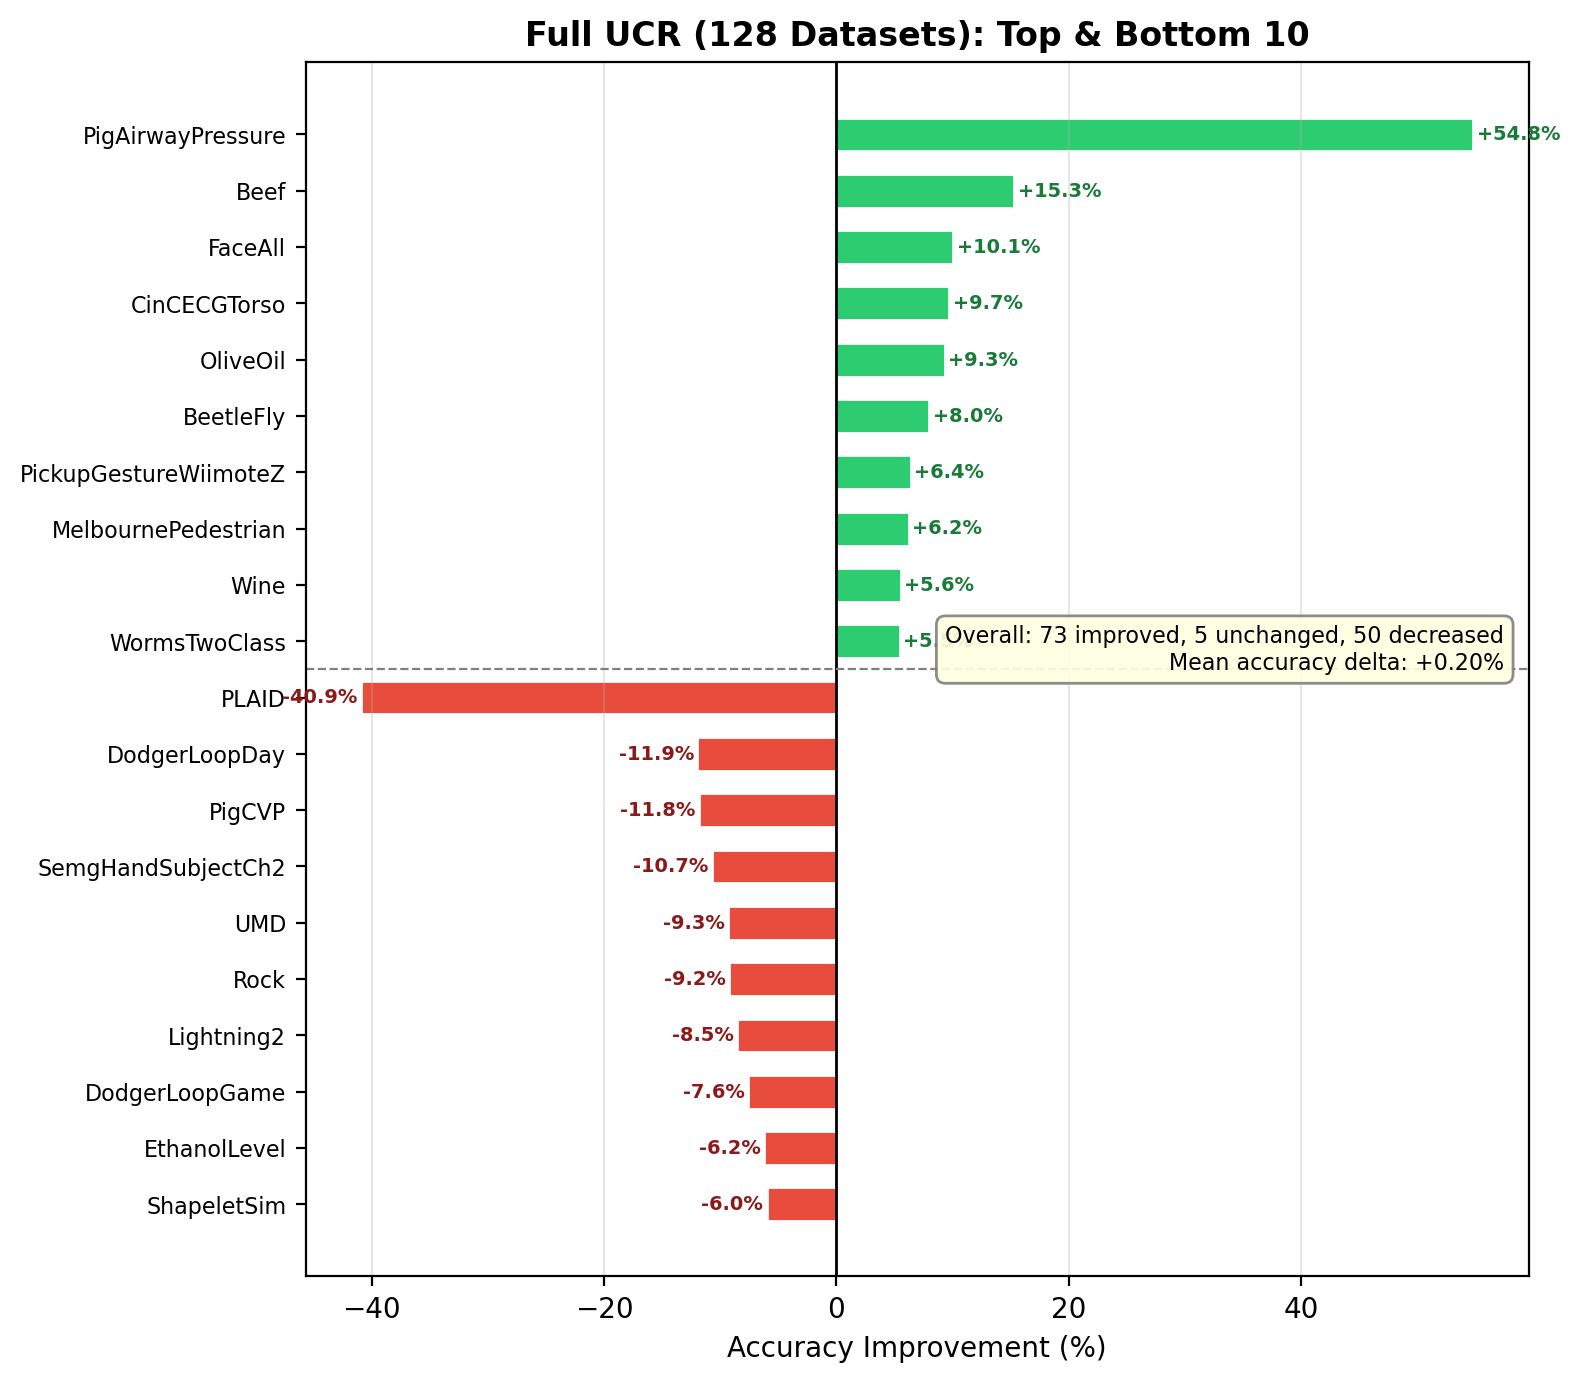
\includegraphics[width=\columnwidth]{plots/full_ucr_improvement.png}
\caption{Per-dataset accuracy improvement across all 128 UCR datasets. The improved configuration (global z-normalization + differenced channel + AdamW) achieved higher accuracy on 73 datasets, with a mean improvement of +0.20\%. The most extreme gains exceeded +50\% (PigAirwayPressure), while the largest decrease was $-$40.9\% (PLAID).}
\label{fig:full_ucr_improvement}
\end{figure}

\begin{figure}[htbh]
\centering
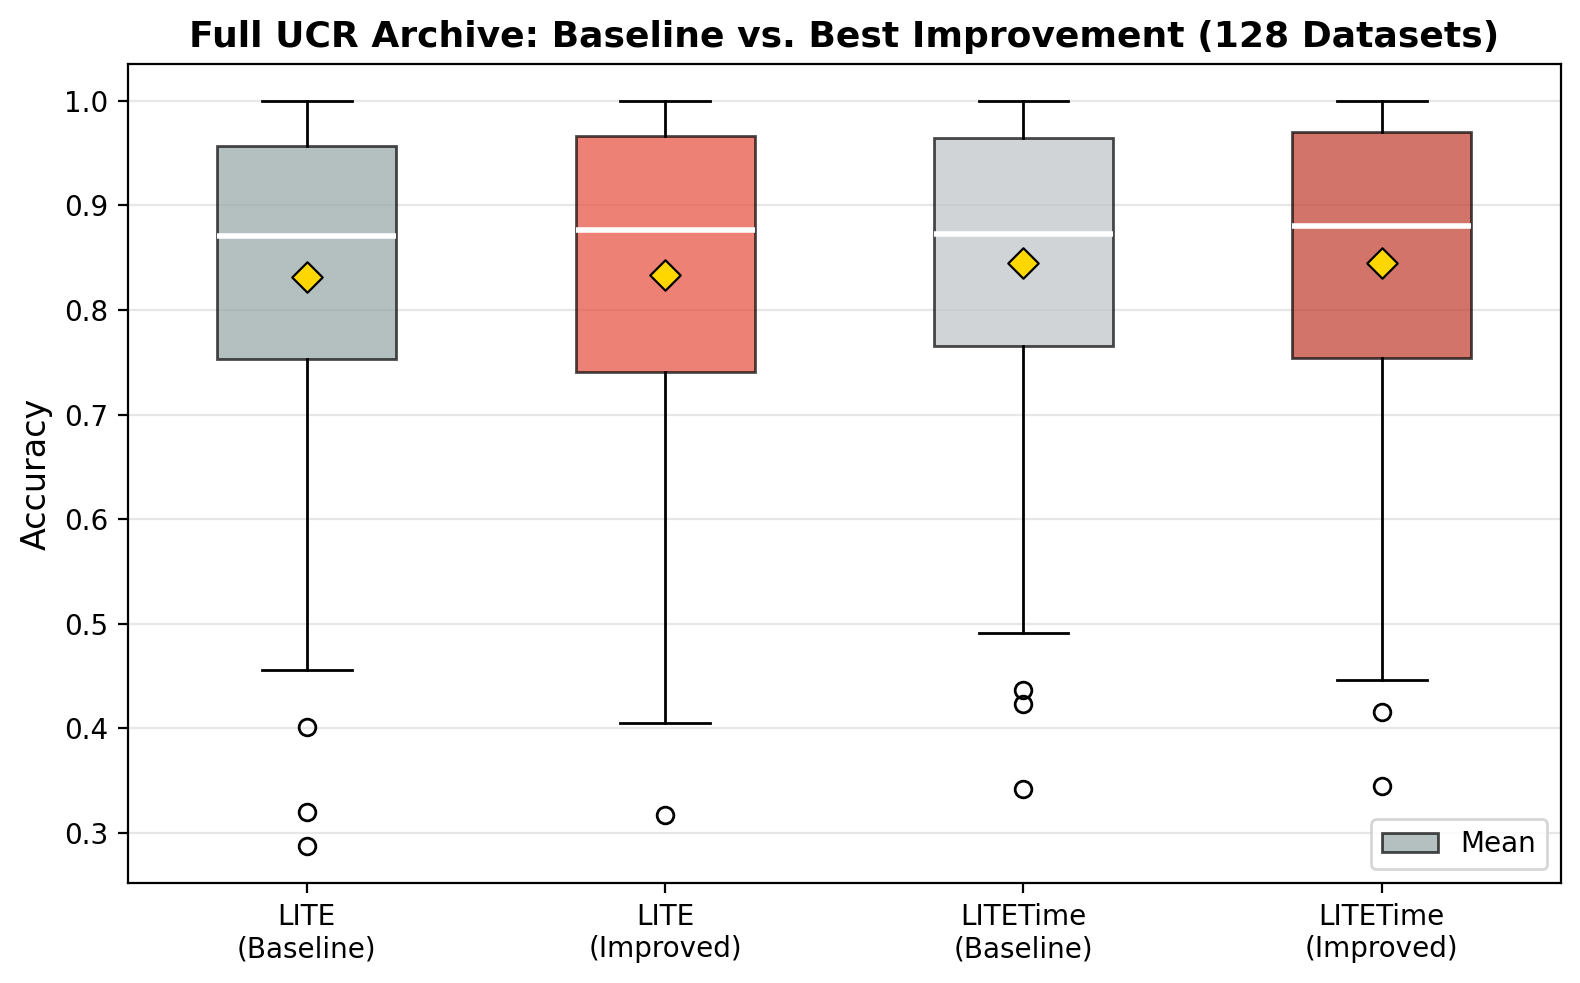
\includegraphics[width=\columnwidth]{plots/full_ucr_boxplot.png}
\caption{Accuracy distribution comparison between baseline and improved configurations across the full 128-dataset UCR archive. The improved LITE configuration shows an upward-shifted distribution with a higher median, while LITETime performance remains essentially unchanged. Gold diamonds indicate mean accuracy values.}
\label{fig:full_ucr_boxplot}
\end{figure}

% ---------------- Discussion ----------------

\section{Discussion}

The results obtained from this study provide several important insights into the behavior and performance characteristics of lightweight deep learning models for time series classification.

First, the successful reproduction of published results confirms the reliability of the original LITETime architecture. Achieving comparable performance values (0.8316 vs. 0.8304) across the full 128-dataset UCR archive demonstrates that the implementation pipeline is robust and consistent across independent environments.

Second, improvement experiments on the fast subset revealed that preprocessing and optimization strategies can significantly influence classification performance. Among all tested configurations, the differenced input channel combined with global z-normalization produced the strongest mean performance gain (+1.30\%). This finding emphasizes the importance of feature engineering in time series analysis.

Third, normalization strategies were found to strongly impact training stability. Global z-normalization produced consistent improvements across datasets (+0.88\%), while global min-max normalization produced less stable results ($-$1.61\%).

Fourth, the combined AdamW + z-normalization experiment demonstrated that optimizer and normalization improvements are complementary. While the overall mean improvement was moderate (+0.32\%), the configuration produced substantial gains on challenging datasets such as Crop (+2.8\%), CricketX (+1.2\%), and BME (+3.3\%), improving accuracy on 20 out of 30 datasets.

Fifth, the full 128-dataset UCR archive evaluation confirmed that improvements generalize beyond the fast subset. The best configuration achieved higher accuracy on 73 out of 128 datasets (57.0\%), with a mean improvement of +0.20\%. The slightly lower delta compared to the fast subset (+1.30\%) is expected, as the full archive includes datasets with fundamentally different characteristics that may not benefit from the same preprocessing strategies.

Sixth, ensemble analysis demonstrated diminishing returns beyond moderate ensemble sizes. This observation suggests that selecting an optimal ensemble size is essential to balance predictive accuracy and computational efficiency.

Additionally, training time analysis confirmed that most improvement configurations achieve improved performance without substantially increasing computational cost. The full UCR evaluation even showed a slight reduction in training time ($-$1.6\%). These results support the practical viability of lightweight architectures such as LITETime in real-world applications.

Overall, the findings demonstrate that meaningful improvements can be achieved through systematic optimization without requiring significant architectural redesign.

% ---------------- Limitations ----------------

\section{Limitations and Future Work}

Although this study produced valuable insights, several limitations should be considered.

First, the most significant accuracy outliers in the full UCR evaluation (PigAirwayPressure at +54.8\% and PLAID at $-$40.9\%) suggest that certain datasets are particularly sensitive to preprocessing and normalization choices, which may introduce instability in aggregate metrics.

Second, the evaluation focused on a limited number of optimization strategies. Future work could explore additional techniques including advanced learning rate schedules, automated hyperparameter optimization, and hybrid architecture extensions.

Third, multivariate experiments demonstrated competitive performance but did not achieve top accuracy compared to transformer-based models. Future research may investigate integrating attention mechanisms into lightweight architectures to enhance cross-channel learning.

Further exploration of energy-efficient model design remains an important direction for continued research.

% ---------------- Conclusion ----------------

\section{Conclusion}

This study successfully reproduced the published LITETime results and validated the reliability of the original architecture. Reproduced performance closely matched reported benchmarks across the full 128-dataset UCR archive (0.8316 vs. 0.8304), confirming the reproducibility of the model across independent environments.

Improvement experiments demonstrated that performance gains can be achieved through targeted optimization strategies without modifying the core architecture. On the 30-dataset fast subset, differenced input channels combined with global z-normalization provided the strongest mean improvement (+1.30\%), followed by learnable filter initialization (+1.18\%) and AdamW with differenced channels (+1.11\%). The combined AdamW + z-normalization experiment further confirmed that optimizer and preprocessing strategies contribute complementary benefits, improving accuracy on 20 out of 30 datasets.

Critically, the best-performing configuration was validated across the complete 128-dataset UCR archive, achieving improved accuracy on 73 out of 128 datasets (57.0\%) with a mean improvement of +0.20\% and no increase in training time. This full-archive validation confirms that the observed improvements generalize beyond the experimental subset.

Ensemble analysis confirmed that moderate ensemble sizes offer an effective balance between performance and computational efficiency. Multivariate evaluation further demonstrated the adaptability of LITE-based architectures across more complex classification tasks.

Overall, the findings highlight the effectiveness of lightweight deep learning architectures for time series classification and reinforce the importance of reproducible experimentation in machine learning research. Lightweight deep learning architectures such as LITETime provide an effective balance between predictive performance and computational efficiency, making them suitable for scalable real-world deployment.

\section*{Work Plan}

The project was completed over an eight-week period with structured milestones to ensure steady progress and timely completion.

\begin{table}[H]
\centering
\caption{Project Timeline}
\begin{tabular}{ll}
\toprule
Phase & Duration \\
\midrule
Paper selection and review & Week 1 \\
Environment setup & Week 2 \\
Dataset preparation & Week 2 \\
Baseline reproduction & Weeks 3--4 \\
Improvement experiments & Weeks 5--6 \\
Visualization and analysis & Week 7 \\
Report writing and revision & Weeks 7--8 \\
Final validation and submission & Week 8 \\
\bottomrule
\end{tabular}
\end{table}



\section*{Team Contributions}

The project was completed collaboratively by all team members.

\textbf{Kiran Meenakshi Sundaram} contributed to dataset preparation, repository development, execution of baseline experiments, generation of visualizations, and report preparation.

\textbf{Jose Ramon Morera Campos} contributed to implementation refinement, optimizer experiments, normalization studies, and evaluation of batch size configurations.

\textbf{Pelayo Garcia Alvarez} contributed to improvement experiments, generation and refinement of result visualizations, multivariate analysis, interpretation of experimental results, and literature review.

All members participated in experiment design, result validation, and report editing.



\section*{Data and Code Availability}

All datasets used in this study are publicly available from the UCR Time Series Classification Archive.

The complete implementation, experiment configurations, generated results, and visualization scripts are available in the public project repository:

\url{https://github.com/jose-r-morera/LITE}

This repository contains all components necessary to reproduce the results presented in this report.

% ---------------- References ----------------

{\footnotesize
\setlength{\itemsep}{0pt}
\setlength{\parskip}{0pt}
\begin{thebibliography}{16}

\bibitem{lite2025}
A. Ismail-Fawaz, M. Devanne, S. Berretti, J. Weber, and G. Forestier,
``Look Into the LITE in Deep Learning for Time Series Classification,'' 
\emph{International Journal of Data Science and Analytics}, 2025.

\bibitem{ucr}
H. Dau \emph{et al.},
``The UCR Time Series Classification Archive,'' 
2018.

\bibitem{fcn}
Z. Wang, W. Yan, and T. Oates,
``Time series classification from scratch with deep neural networks: A strong baseline,'' 
\emph{IJCNN}, 2017.

\bibitem{resnet}
Z. Wang \emph{et al.},
``Residual networks for time series classification,'' 
2017.

\bibitem{inceptiontime}
H. Ismail-Fawaz \emph{et al.},
``InceptionTime: Finding AlexNet for time series classification,'' 
\emph{Data Mining and Knowledge Discovery}, 2020.

\bibitem{adamw}
I. Loshchilov and F. Hutter,
``Decoupled weight decay regularization,'' 
\emph{ICLR}, 2019.

\bibitem{rocket}
A. Dempster, F. Petitjean, and G. Webb,
``ROCKET: Exceptionally fast and accurate time series classification,'' 
2020.

\bibitem{minirocket}
A. Dempster, D. Schmidt, and G. Webb,
``MiniROCKET: A very fast deterministic transform,'' 
2021.

\bibitem{shapelet}
J. Lines \emph{et al.},
``Time series classification with shapelets,'' 
2012.

\bibitem{convtran}
N. Foumani \emph{et al.},
``Improving position encoding of transformers for multivariate time series classification,'' 
2023.

\end{thebibliography}
}

\end{document}